\chapter{Auswahl des Materials}

\begin{figure}[h]
  \centering
  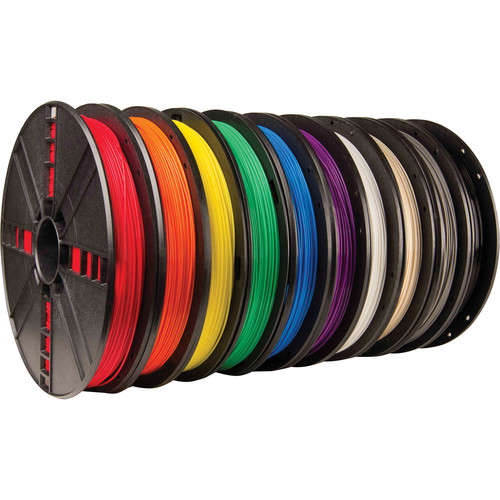
\includegraphics[width=10cm]{kapitel2/filament}
  \caption{Filamentspulen}
  \source{\url{https://www.bhphotovideo.com/c/product/1070383-REG/makerbot_mp06572_1_75mm_pla_filament_large.html}}
  \label{Kap2:Filament}
\end{figure}

\section{PLA}
\ac{PLA} ist das gängigste Material im 3D-Druck Hobbybereich bei einer Drucktemperatur von ca. 210\degree C. Preislich liegt es mit ca. 25€/kg im günstigen Bereich. Aufgrund seiner Eigenschaften\footnote{PLA Materialeigenschaften nach \cite{ULABS2017}} ist es sehr einfach in jedem Einsteiger-3D-Drucker zu verarbeiten. Es ist vergleichsweise leicht und umweltfreundlich, da es nicht aus Erdöl hergestellt wird und biologisch schneller abbaubar ist als andere Kunststoffe\footnote{Nach \cite{Tokiwa2009}}. Auch ist es durch die weite Verbreitung gerade im 3D-Druck Bereich sehr günstig.

Punkte die gegen den Einsatz von \ac{PLA} sprechen sind hingegen die schwache mechanische Belastbarkeit und Temperaturstabilität, da \ac{PLA} nach der \ac{VST} nur bis ca. 54\degree C fest ist.

Außerhalb des 3D-Druckes wird \ac{PLA} vor allem für Verpackungen eingesetzt, da hier die mechanische Belastbarkeit eine untergeordnete Rolle spielt und die Umweltfreundlichkeit im Vordergrund steht.

\begin{figure}[h]
  \centering
  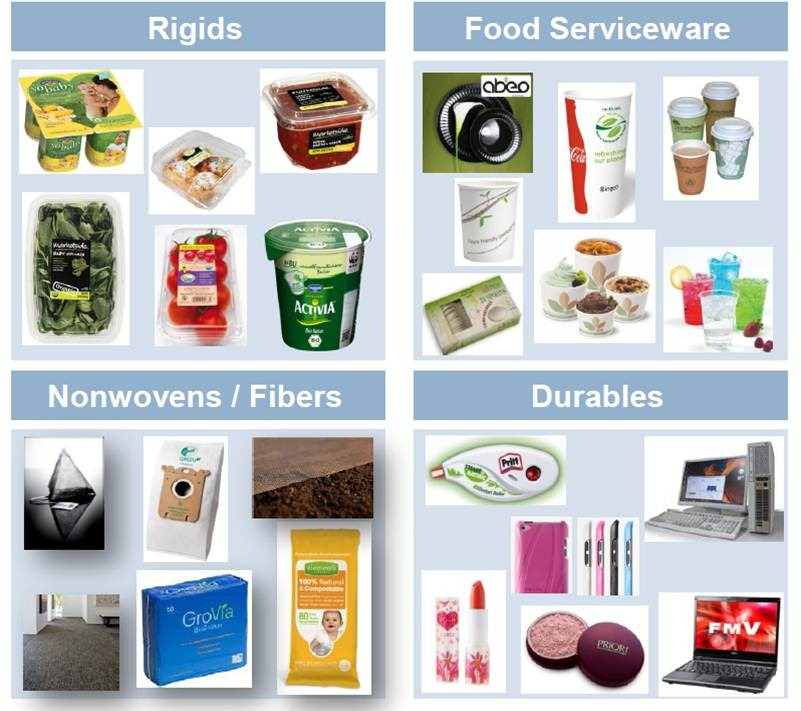
\includegraphics[width=10cm]{kapitel2/pla}
  \caption{Nutzungsgebiete von PLA}
  \source{\url{https://polymerinnovationblog.com/poly-lactic-acid-pla-is-gaining-traction-in-the-market/}}
  \label{Kap2:PLAEinsatz}
\end{figure}

\section{ABS}
Neben \ac{PLA} ist \ac{ABS} ein weiteres gängiges Material, welches jedoch vor allem im Profi-Bereich eingesetzt wird, da dort die Materialanforderungen häufig höher sind und es aufgrund seiner Eigenschaften\footnote{ABS Materialeigenschaften nach \cite{ULPLA2017}} höhere Anforderungen an den 3D-Drucker stellt. Dafür besitzt es jedoch eine sehr hohe Festigkeit und ist auch für mechanisch belastete Teile geeignet. Gedruckt wird es bei ca. 275\degree C und preislich liegt es mit ca. 25€/kg im günstigen Bereich.

Die hohen Anforderungen sind jedoch auch der Hauptpunkte, welche gegen einen Einsatz von \ac{ABS} sprechen, da das Material sehr zu \textit{Warping}\footnote{Verformung des Materials bei zu schneller Abkühlung} neigt und deshalb in einer geschlossenen Kammer und mit beheiztem Druckbett gedruckt werden muss, welche nur wenige günstige 3D-Drucker besitzen. Es ist biologisch vergleichsweise zu \ac{PLA} nicht so schnell abbaubar und weniger umweltfreundlich, da es aus Erdöl hergestellt wird, zudem entstehen während des Druckvorgangs gesundheitsschädliche Mikropartikel\footnote{\cite{Azimi2016}}.

Außerhalb des 3D-Druckes wird \ac{ABS} vor allem für Spielzeug und Gehäuse von Haushaltsgeräten verwendet.

\begin{figure}[h]
  \centering
  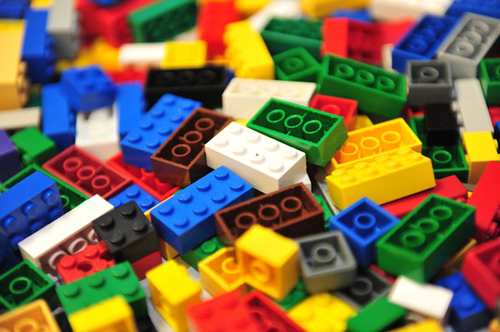
\includegraphics[width=10cm]{kapitel2/abs}
  \caption{LEGO-Bausteine aus ABS}
  \source{\url{https://27gen.com/2016/04/06/lego-bricks-toys-for-kids-lessons-for-adults/}}
  \label{Kap2:ABSLego}
\end{figure}

\section{Weitere Alternativen}

Nach den oben Genannten gibt unzählige weitere Materialien, welche sich zum 3D-Druck eignen. Im Folgenden werden noch zwei weitere Alternativen vorgestellt, welche aufgrund ihrer Eigenschaften für sehr spezielle Anwendungsfälle geeignet sind.

\subsection{HIPS}
\ac{HIPS} hat ähnliche Eigenschaften\footnote{HIPS Materialeigenschaften nach \cite{ZHIPS2016}} wie \ac{ABS}, bietet jedoch eine wesentlich höhere Schlagfestigkeit, wodurch es \zb für Gehäuse welche starken Stößen ausgesetzt sind verwendet werden kann.

Auch eignet es sich für das Drucken von Stützmaterial, da es in bestimmten Chemikalien aufgelöst werden kann\footnote{\cite{Hearon2013}}. Preislich liegt es dabei mit ca. 35€/kg im Mittelfeld.

\subsection{Composit-Materialien}
Bei Composit-Materialien handelt es sich um mit Verbundstoffen verstärkte Kunststoffe. Beispielsweise kann \ac{ABS} mit Kohlestofffasern oder \ac{PLA} mit Graphen verstärkt werden. Hierdurch verbessert sich die Materialstärke\footnote{Composit Materialeigenschaften nach \cite{Zhenyu2016}} um über 20\% und kann damit sogar eine Festigkeit ähnlich der von manchen Metallen erreichen.

Allerdings sind Composit-Materialien mit ca. 80€/kg preislich weit im oberen Bereich und nutzen aufgrund der Partikel den Druckkopf wesentlich schneller ab, weshalb ein speziell gehärteter Druckkopf hier sinnvoll ist.

\begin{figure}[h]
  \centering
  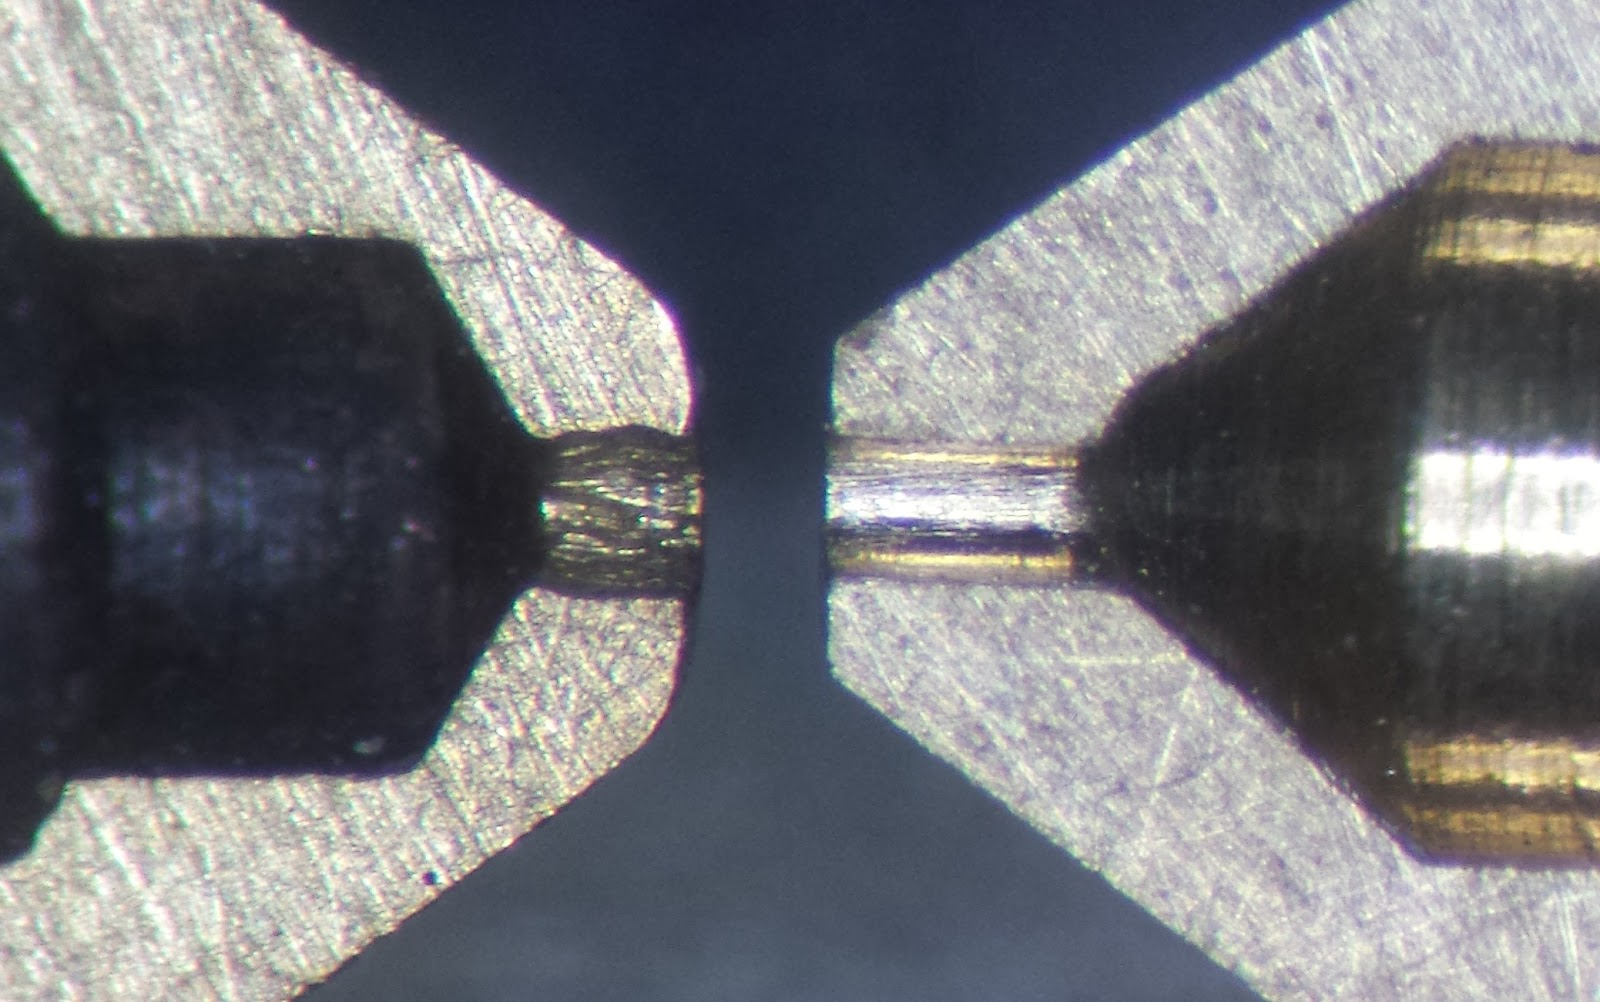
\includegraphics[width=5cm]{kapitel2/carbonnozzle}
  \caption{Links: Druckkopf nach Druck von Kohlenstoff-Materialien -- Rechts: Neuer Druckkopf}
  \source{\url{http://e3d-online.com/is-carbon-killing-your-nozzle}}
  \label{Kap2:CompositNozzle}
\end{figure}